\section{Практическая часть}
\subsection{Примеры}
Первый в мире интерактивный программируемый движок трассировки лучей использует мощности параллельных видеопроцессоров NVIDIA; с его помощью разработчики могут легко достичь нового уровня реализма в своих приложениях, используя традиционный язык С. OptiX может значительно ускорить визуализацию методом трассировки лучей в ряде направлений, включая: создание фотореалистичных моделей, дизайн автомобилей, разработка музыкальных инструментов и оптических систем, расчеты емкости и исследования радиации.
\begin{figure}[h!]
\center{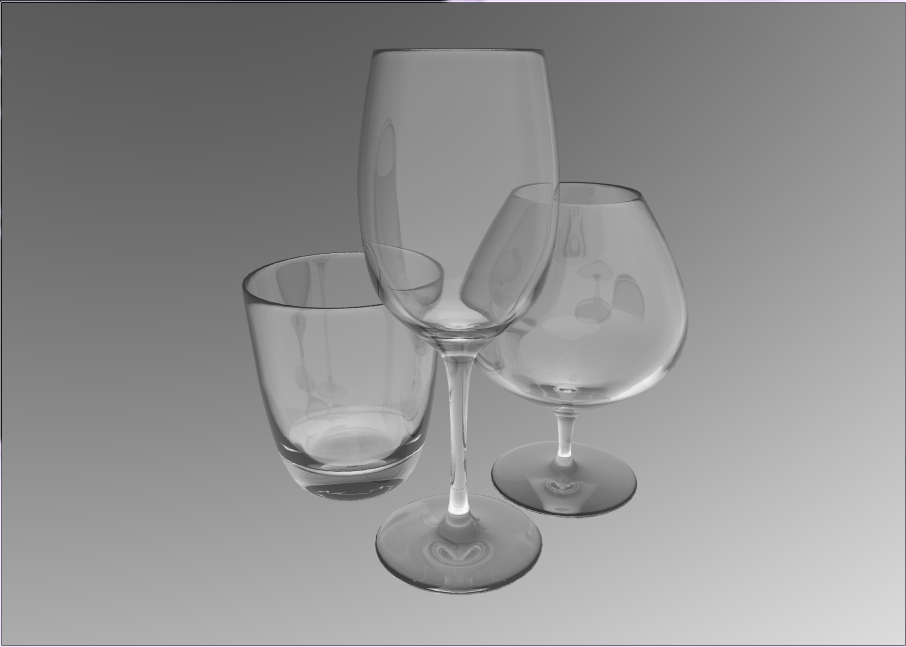
\includegraphics[width=0.5\linewidth]{glass.png}}
\caption{пример 1.}
\label{glass}
\end{figure}
 Сложные задачи дизайна, такие как передача игры отражений и преломлений на поверхностях и внутри стекла, могут быть реализованы в реальном времени благодаря использованию ускорения движка OptiX на процессорах NVIDIA. Это выдающееся достижение, как для разработчиков, так и для дизайнеров.
\begin{figure}[h!]
\center{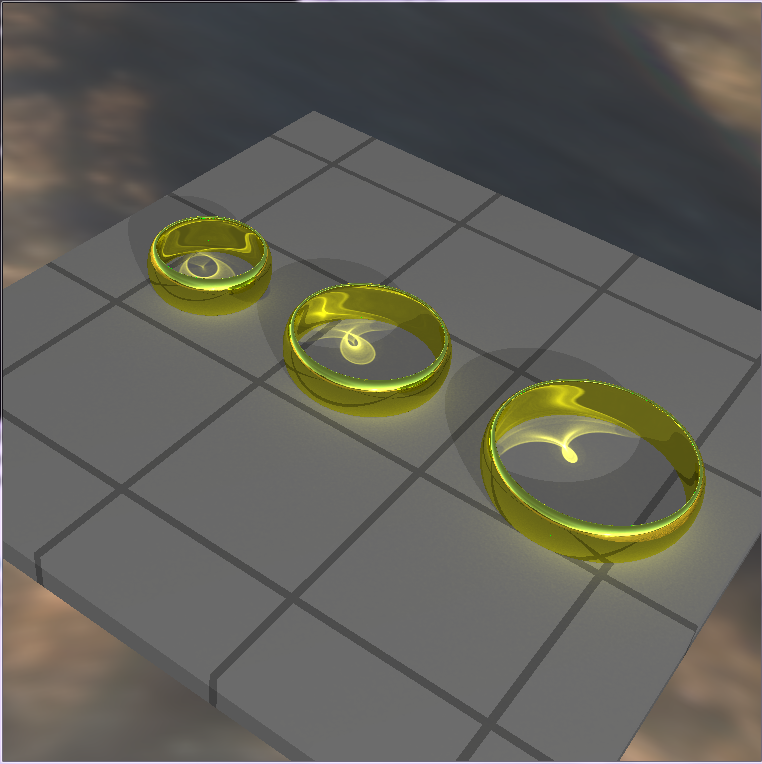
\includegraphics[width=0.5\linewidth]{map.png}}
\caption{Пример 2.}
\label{map}
\end{figure}
 Мир расчетов переместился от вычислений только лишь на процессоре к уравновешенной совместной обработке на CPU и GPU. Движки ускорения приложения от NVIDIA вооружают разработчиков инструментами, в которых они нуждаются для осуществления дальнейшего коренного изменения, как в области графики в реальном времени, так и сложного анализа данных. В отличие от привычных визуализаторов, OptiX является гибкой платформой, позволяющей разработчикам быстро создавать то, что они хотят: движок использует гибридный подход, объединяя оба метода (трассировки лучей и растеризации), для достижения равновесия между реализмом и скоростью работы. 
\subsection{Выполнение работы}
\begin{verbatim}
#include <optixu/optixpp_namespace.h>
#include <optixu/optixu_math_namespace.h>
#include <optixu/optixu_aabb_namespace.h>
#include <sutil.h>
#include <GLUTDisplay.h>
#include <PlyLoader.h>
#include <ObjLoader.h>
#include "commonStructs.h"
#include <string>
#include <iostream>
#include <fstream>
#include <cstdlib>
#include <cstring>
#include "random.h"
#include "MeshScene.h"

using namespace optix;

class MeshViewer : public MeshScene
{
public:
  enum ShadeMode
  {
    SM_PHONG=0,
    SM_AO,
    SM_NORMAL,
    SM_ONE_BOUNCE_DIFFUSE,
    SM_AO_PHONG
  };
  enum CameraMode
  {
    CM_PINHOLE=0,
    CM_ORTHO
  };
    MeshViewer();
  // Setters for controlling application behavior
  void setShadeMode( ShadeMode mode ) { m_shade_mode = mode;}
  void setCameraMode( CameraMode mode ) { m_camera_mode = mode;}
  void setAORadius( float ao_radius ) { m_ao_radius = ao_radius;}
  void setAOSampleMultiplier(
   int ao_sample_mult ) { m_ao_sample_mult = ao_sample_mult; }
  void setLightScale( float light_scale ) { m_light_scale = light_scale;}
  void setAA( bool onoff ) { m_aa_enabled = onoff;}
  void setAnimation( bool anim ) { m_animation = anim;}

  virtual void   initScene( InitialCameraData& camera_data );
  virtual void   doResize( unsigned int width, unsigned int height );
  virtual void   trace( const RayGenCameraData& camera_data );
  virtual void   cleanUp();
  virtual bool   keyPressed(unsigned char key, int x, int y);
  virtual Buffer getOutputBuffer();

private:
  void initContext();
  void initLights();
  void initMaterial();
  void initGeometry();
  void initCamera( InitialCameraData& cam_data );
  void preprocess();
  void resetAccumulation();
  void genRndSeeds( unsigned int width, unsigned int height );

  CameraMode    m_camera_mode;
  ShadeMode  m_shade_mode;
  bool    m_aa_enabled;
  float    m_ao_radius;
  int       m_ao_sample_mult;
  float    m_light_scale;

  Material  m_material;
  Aabb      m_aabb;
  Buffer     m_rnd_seeds;
  Buffer     m_accum_buffer;
  bool       m_accum_enabled;

  float       m_scene_epsilon;
  int          m_frame;
  bool        m_animation;
};
MeshViewer::MeshViewer():
  MeshScene ( false, false, false ),
  m_camera_mode ( CM_PINHOLE ),
  m_shade_mode ( SM_PHONG ),
  m_aa_enabled ( false ),
  m_ao_radius ( 1.0f ),
  m_ao_sample_mult ( 1 ),
  m_light_scale ( 1.0f ),
  m_accum_enabled ( false ),
  m_scene_epsilon ( 1e-4f ),
  m_frame ( 0 ),
  m_animation ( false )
{
}
void MeshViewer::initScene( InitialCameraData& camera_data )
{
  initContext();
  initLights();
  initMaterial();
  initGeometry();
  initCamera( camera_data );
  preprocess();
}
void MeshViewer::initContext()
{
  m_context->setRayTypeCount( 3 );
  m_context->setEntryPointCount( 1 );
  m_context->setStackSize( 1180 );

  m_context[ "radiance_ray_type" ]->setUint( 0u );
  m_context[ "shadow_ray_type" ]->setUint( 1u );
  m_context[ "max_depth" ]->setInt( 5 );
  m_context[ "ambient_light_color" ]->setFloat( 0.2f, 0.2f, 0.2f );
  m_context[ "output_buffer" ]->set(
   createOutputBuffer(RT_FORMAT_UNSIGNED_BYTE4, WIDTH, HEIGHT) );
  m_context[ "jitter_factor" ]->setFloat( m_aa_enabled ? 1.0f : 0.0f );
  
  m_accum_enabled = m_aa_enabled ||
                   m_shade_mode == SM_AO ||
                   m_shade_mode == SM_ONE_BOUNCE_DIFFUSE ||
                   m_shade_mode == SM_AO_PHONG;
 // Ray generation program setup
  const std::string camera_name = m_camera_mode == CM_PINHOLE ?
   "pinhole_camera" : "orthographic_camera"; 
  const std::string camera_file = m_accum_enabled? "accum_camera.cu" :
                         m_camera_mode == CM_PINHOLE ?
                       "pinhole_camera.cu"  : "orthographic_camera.cu";

  if( m_accum_enabled ) {
    // The raygen program needs accum_buffer
    m_accum_buffer = m_context->createBuffer(
     RT_BUFFER_INPUT_OUTPUT | RT_BUFFER_GPU_LOCAL, RT_FORMAT_FLOAT4,
                                            WIDTH, HEIGHT );
    m_context["accum_buffer"]->set( m_accum_buffer );
    resetAccumulation();
  }
  const std::string camera_ptx  = ptxpath( "sample6", camera_file );
  Program ray_gen_program = m_context->createProgramFromPTXFile( 
  camera_ptx, camera_name );
  m_context->setRayGenerationProgram( 0, ray_gen_program );
  // Exception program
  const std::string except_ptx  = ptxpath( "sample6", camera_file );
  m_context->setExceptionProgram( 0, m_context->createProgramFromPTXFile( 
  except_ptx, "exception" ) );
  m_context[ "bad_color" ]->setFloat( 0.0f, 1.0f, 0.0f );
 // Miss program 
  const std::string miss_ptx = ptxpath( "sample6", "constantbg.cu" );
  m_context->setMissProgram( 0, m_context->createProgramFromPTXFile( 
  miss_ptx, "miss" ) );
  m_context[ "bg_color" ]->setFloat(  0.34f, 0.55f, 0.85f );
}
void MeshViewer::initLights()
{
  // Lights buffer
  BasicLight lights[] = {
    { make_float3( -60.0f,  30.0f, -120.0f ),
     make_float3( 0.2f, 0.2f, 0.25f )*m_light_scale, 0, 0 },
    { make_float3( -60.0f,   0.0f,  120.0f ),
     make_float3( 0.1f, 0.1f, 0.10f )*m_light_scale, 0, 0 },
    { make_float3(  60.0f,  60.0f,   60.0f ), 
    make_float3( 0.7f, 0.7f, 0.65f )*m_light_scale, 1, 0 }
  };
 Buffer light_buffer = m_context->createBuffer(RT_BUFFER_INPUT);
  light_buffer->setFormat(RT_FORMAT_USER);
  light_buffer->setElementSize(sizeof( BasicLight ) );
  light_buffer->setSize( sizeof(lights)/sizeof(lights[0]) );
  memcpy(light_buffer->map(), lights, sizeof(lights));
  light_buffer->unmap();

  m_context[ "lights" ]->set( light_buffer );
}
void MeshViewer::initMaterial()
{
  switch( m_shade_mode ) {
    case SM_PHONG: {
      // Use the default obj_material created by ObjLoader
      break;
    }
   case SM_NORMAL: {
      const std::string ptx_path = ptxpath("sample6", "normal_shader.cu");
      m_material = m_context->createMaterial();
      m_material->setClosestHitProgram(
       0, m_context->createProgramFromPTXFile( ptx_path, "closest_hit_radiance" ) );
      break;
    }
    case SM_AO: {
      const std::string ptx_path = ptxpath("sample6", "ambocc.cu");
      m_material = m_context->createMaterial();
      m_material->setClosestHitProgram(
       0, m_context->createProgramFromPTXFile( ptx_path, "closest_hit_radiance" ) );
      m_material->setAnyHitProgram(
       1, m_context->createProgramFromPTXFile( ptx_path, "any_hit_occlusion" ) );    
      break;
    }  
    case SM_ONE_BOUNCE_DIFFUSE: {
      const std::string ptx_path = ptxpath("sample6", "one_bounce_diffuse.cu");
      m_material = m_context->createMaterial();
      m_material->setClosestHitProgram(
       0, m_context->createProgramFromPTXFile( ptx_path, "closest_hit_radiance" ) );
      m_material->setAnyHitProgram    (
       1, m_context->createProgramFromPTXFile( ptx_path, "any_hit_shadow" ) );
      break;
    }
    case SM_AO_PHONG: {
      const std::string ptx_path = ptxpath("sample6", "ambocc.cu");
      m_material = m_context->createMaterial();
      m_material->setClosestHitProgram( 
      0, m_context->createProgramFromPTXFile( 
      ptx_path, "closest_hit_radiance_phong_ao" ) );
      m_material->setAnyHitProgram(
       1, m_context->createProgramFromPTXFile( ptx_path, "any_hit_shadow" ) );
      m_material->setAnyHitProgram(
       2, m_context->createProgramFromPTXFile( ptx_path, "any_hit_occlusion" ) );
      m_context["Kd"]->setFloat(1.0f);
      m_context["Ka"]->setFloat(0.6f);
      m_context["Ks"]->setFloat(0.0f);
      m_context["Kr"]->setFloat(0.0f);
      m_context["phong_exp"]->setFloat(0.0f);
      break;
    }
  }
  if( m_accum_enabled ) {
    genRndSeeds( WIDTH, HEIGHT );
  }
}
void MeshViewer::initGeometry()
{
  double start, end;
  sutilCurrentTime(&start);

  m_geometry_group = m_context->createGeometryGroup();
  if( ObjLoader::isMyFile( m_filename.c_str() ) ) {
    // Load OBJ model 
    ObjLoader* loader = 0;
    if( m_shade_mode == SM_NORMAL || m_shade_mode == SM_AO |
    | m_shade_mode == SM_AO_PHONG ) {
      loader = new ObjLoader( m_filename.c_str(), m_context, m_geometry_group,
       m_material, false,  m_accel_builder.c_str(), m_accel_traverser.c_str(),
        m_accel_refine.c_str(), m_accel_large_mesh );
    } else if ( m_shade_mode == SM_ONE_BOUNCE_DIFFUSE ) {
      loader = new ObjLoader( m_filename.c_str(), m_context, m_geometry_group,
       m_material, true,  m_accel_builder.c_str(), m_accel_traverser.c_str(), 
       m_accel_refine.c_str(), m_accel_large_mesh );
    } else {
      loader = new ObjLoader( m_filename.c_str(), m_context, m_geometry_group,
       m_accel_builder.c_str(), m_accel_traverser.c_str(),
        m_accel_refine.c_str(), m_accel_large_mesh );
    }
    loader->load();
    m_aabb = loader->getSceneBBox();
    delete loader;
  } else if( PlyLoader::isMyFile( m_filename ) ) {
    // Load PLY model 
    PlyLoader loader( m_filename, m_context, m_geometry_group, m_material,
     m_accel_builder.c_str(), m_accel_traverser.c_str(), m_accel_refine.c_str(), 
     m_accel_large_mesh );
    loader.load();
    m_aabb = loader.getSceneBBox();
  } else {
    std::cerr << "Unrecognized model file extension '" <<
     m_filename << "'" << std::endl;
    exit( 0 );
  }
  loadAccelCache();
 
  m_context[ "top_object" ]->set( m_geometry_group );
  m_context[ "top_shadower" ]->set( m_geometry_group );

  sutilCurrentTime(&end);
  std::cerr << "Time to load " << (m_accel_large_mesh ? "and cluster " : "") <<
   "geometry: " << end-start << " s.\n";
}
void MeshViewer::initCamera( InitialCameraData& camera_data )
{
  // Set up camera
  float max_dim  = m_aabb.maxExtent();
  float3 eye     = m_aabb.center();
  eye.z         += 2.0f * max_dim;

  camera_data = InitialCameraData( eye,  // eye
                                   m_aabb.center(), // lookat
                                   make_float3( 0.0f, 1.0f, 0.0f ), // up
                                   30.0f );                         // vfov

  // Declare camera variables. 
  m_context[ "eye"]->setFloat( make_float3( 0.0f, 0.0f, 0.0f ) );
  m_context[ "U"  ]->setFloat( make_float3( 0.0f, 0.0f, 0.0f ) );
  m_context[ "V"  ]->setFloat( make_float3( 0.0f, 0.0f, 0.0f ) );
  m_context[ "W"  ]->setFloat( make_float3( 0.0f, 0.0f, 0.0f ) );
}
void MeshViewer::preprocess()
{
  // Settings which rely on previous initialization
  m_scene_epsilon = 1.e-4f * m_aabb.maxExtent();
  m_context[ "scene_epsilon"      ]->setFloat( m_scene_epsilon );
  m_context[ "occlusion_distance" ]->setFloat(
   m_aabb.maxExtent() * 0.3f * m_ao_radius );

  // Prepare to run 
  m_context->validate();
  double start, end_compile, end_AS_build;
  sutilCurrentTime(&start);
  m_context->compile();
  sutilCurrentTime(&end_compile);
  std::cerr << "Time to compile kernel: "<<end_compile-start<<" s.\n";
  m_context->launch(0,0);
  sutilCurrentTime(&end_AS_build);
  std::cerr << "Time to build AS: "<<end_AS_build-end_compile<<" s.\n";
  // Save cache file
  saveAccelCache();
}
bool MeshViewer::keyPressed(unsigned char key, int x, int y)
{
   switch (key)
   {
     case 'e':
       m_scene_epsilon *= .1f;
       std::cerr << "scene_epsilon: " << m_scene_epsilon << std::endl;
       m_context[ "scene_epsilon" ]->setFloat( m_scene_epsilon );
       return true;
     case 'E':
       m_scene_epsilon *= 10.0f;
       std::cerr << "scene_epsilon: " << m_scene_epsilon << std::endl;
       m_context[ "scene_epsilon" ]->setFloat( m_scene_epsilon );
       return true;
   }
   return false;
}
void MeshViewer::doResize( unsigned int width, unsigned int height )
{
  // output_buffer resizing handled in base class
  if( m_accum_enabled ) {
    m_accum_buffer->setSize( width, height );
    m_rnd_seeds->setSize( width, height );
    genRndSeeds( width, height );
    resetAccumulation();
  }
}
void MeshViewer::trace( const RayGenCameraData& camera_data )
{
  if (m_animation && GLUTDisplay::isBenchmark() ) {
    static float angleU = 0.0f, angleV = 0.0f, scale = 1.0f,
     dscale = 0.96f, backside = 0.0f;
    static int phase = 0, accumed_frames = 0;
    const float maxang = M_PIf * 0.2f;
    const float rotvel = M_2_PIf*0.1f;
    float3 c = m_aabb.center();
    float3 e = camera_data.eye;

    Matrix3x3 m = make_matrix3x3(
    Matrix4x4::rotate(angleV + backside, normalize(camera_data.V)) * 
      Matrix4x4::rotate(angleU, normalize(camera_data.U)) * Matrix4x4::scale(
      make_float3(scale, scale, scale)));

    if( !m_accum_enabled || accumed_frames++ > 5 ) {
      switch(phase) {
      case 0: angleV += rotvel; if(angleV > maxang)
       { angleV =  maxang; phase++; } break;
      case 1: angleU += rotvel; if(angleU > maxang)
       { angleU =  maxang; phase++; } break;
      case 2: angleV -= rotvel; if(angleV <-maxang)
       { angleV = -maxang; phase++; } break;
      case 3: angleU -= rotvel; if(angleU <-maxang)
       { angleU = -maxang; phase=0; } break;
      }
      scale *= dscale;
      if(scale < 0.1f) { dscale = 1.0f / dscale; backside = M_PIf - backside; }
      if(scale > 1.0f) { dscale = 1.0f / dscale; }

      accumed_frames = 0;
      m_camera_changed = true;
    }

    m_context["eye"]->setFloat( c-m*(c-e) );
    m_context["U"]->setFloat( m*camera_data.U );
    m_context["V"]->setFloat( m*camera_data.V );
    m_context["W"]->setFloat( m*camera_data.W );
  } else {
    m_context["eye"]->setFloat( camera_data.eye );
    m_context["U"]->setFloat( camera_data.U );
    m_context["V"]->setFloat( camera_data.V );
    m_context["W"]->setFloat( camera_data.W );
  }
  Buffer buffer = m_context["output_buffer"]->getBuffer();
  RTsize buffer_width, buffer_height;
  buffer->getSize( buffer_width, buffer_height );

  if( m_accum_enabled && !m_camera_changed ) {
    m_context["sqrt_occlusion_samples"]->setInt( 3 * m_ao_sample_mult );
    m_context["sqrt_diffuse_samples"]->setInt( 3 );
  }
  m_context->launch( 0, static_cast<unsigned int>(buffer_width),
   static_cast<unsigned int>(buffer_height) );

  if( m_accum_enabled ) {
      ++m_frame;
    if( m_camera_changed ) {
      m_camera_changed = false;
      resetAccumulation();
    }
    m_context["frame"]->setInt( m_frame );
  }
}
void MeshViewer::cleanUp()
{
  SampleScene::cleanUp();
}
Buffer MeshViewer::getOutputBuffer()
{
  return m_context["output_buffer"]->getBuffer();
}
void MeshViewer::resetAccumulation()
{
  m_frame = 0;
  m_context[ "frame"]->setInt( m_frame );
  m_context[ "sqrt_occlusion_samples" ]->setInt( 1 * m_ao_sample_mult );
  m_context[ "sqrt_diffuse_samples"   ]->setInt( 1 );
}
void MeshViewer::genRndSeeds( unsigned int width, unsigned int height )
{
  // Init random number buffer if necessary.
  if( m_rnd_seeds.get() == 0 ) {
    m_rnd_seeds = m_context->createBuffer(
     RT_BUFFER_INPUT_OUTPUT | RT_BUFFER_GPU_LOCAL, 
     RT_FORMAT_UNSIGNED_INT, WIDTH, HEIGHT);
    m_context["rnd_seeds"]->setBuffer(m_rnd_seeds);
  }
  unsigned int* seeds = static_cast<unsigned int*>( m_rnd_seeds->map() );
  fillRandBuffer(seeds, width*height);
  m_rnd_seeds->unmap();
}
void printUsageAndExit( const std::string& argv0, bool doExit = true )
{
  std::cerr
    << "Usage  : " << argv0 << " [options]\n"
    << "App options:\n"
    << "  -h  | --help                               
    << "  -o  | --obj <obj_file>                    
    << "  -c  | --cache                              
    << "  -a  | --ao-shade                              
    << "  -ap | --ao-phong-shade                    
    << "  -aa | --antialias                          
    << "  -n  | --normal-shade                   
    << "  -i  | --diffuse-shade                    
    << "  -O  | --ortho                              
    << "  -r  | --ao-radius <scale>              
    << "  -m  | --ao-sample-mult <n>             
    << "  -l  | --light-scale <scale>          
    << "        --large-mesh                 
    << "        --animation                    
    << "        --trav <name>          
    << "        --build <name>       
    << "        --refine <n>         
    << std::endl;
  GLUTDisplay::printUsage();

  std::cerr
    << "App keystrokes:\n"
    << "  e Decrease scene epsilon size (used for shadow ray offset)\n"
    << "  E Increase scene epsilon size (used for shadow ray offset)\n"
    << std::endl;

  if ( doExit ) exit(1);
}
int main( int argc, char** argv ) 
{
  GLUTDisplay::init( argc, argv );
  
  GLUTDisplay::contDraw_E draw_mode = GLUTDisplay::CDNone; 
  MeshViewer scene;
  scene.setMesh( (std::string( sutilSamplesDir() ) +
   "/simpleAnimation/cow.obj").c_str() );

  for ( int i = 1; i < argc; ++i ) {
    std::string arg( argv[i] );
    if ( arg == "-c" || arg == "--cache" ) {
      scene.setAccelCaching( true );
    } else if( arg == "-n" || arg == "--normal-shade" ) {
      scene.setShadeMode( MeshViewer::SM_NORMAL );
    } else if( arg == "-a" || arg == "--ao-shade" ) {
      scene.setShadeMode( MeshViewer::SM_AO);
      draw_mode = GLUTDisplay::CDProgressive;
    } else if( arg == "-i" || arg == "--diffuse-shade" ) {
      scene.setShadeMode( MeshViewer::SM_ONE_BOUNCE_DIFFUSE );
      draw_mode = GLUTDisplay::CDProgressive;
    } else if( arg == "-ap" || arg == "--ao-phong-shade" ) {
      scene.setShadeMode( MeshViewer::SM_AO_PHONG );
      draw_mode = GLUTDisplay::CDProgressive;
    } else if( arg == "-aa" || arg == "--antialias" ) {
      scene.setAA( true );
      draw_mode = GLUTDisplay::CDProgressive;
    } else if( arg == "-O" || arg == "--ortho" ) {
      scene.setCameraMode( MeshViewer::CM_ORTHO );
    } else if( arg == "-h" || arg == "--help" ) {
      printUsageAndExit( argv[0] ); 
    } else if( arg == "-o" || arg == "--obj" ) {
      if ( i == argc-1 ) {
        printUsageAndExit( argv[0] );
      }
      scene.setMesh( argv[++i] );
    } else if( arg == "--trav" ) {
      if ( i == argc-1 ) {
        printUsageAndExit( argv[0] );
      }
      scene.setTraverser( argv[++i] );
    } else if( arg == "--build" ) {
      if ( i == argc-1 ) {
        printUsageAndExit( argv[0] );
      }
      scene.setBuilder( argv[++i] );
    } else if( arg == "--refine" ) {
      if ( i == argc-1 ) {
        printUsageAndExit( argv[0] );
      }
      scene.setRefine( argv[++i] );
    } else if( arg == "--kd" ) {  
      scene.setBuilder( "TriangleKdTree" );
      scene.setTraverser( "KdTree" );
    } else if( arg == "--lbvh" ) { 
      scene.setBuilder( "Lbvh" );
    } else if( arg == "--bvh" ) {
      scene.setBuilder( "Bvh" );
    } else if( arg == "--large-mesh" ) {
      scene.setLargeMesh( true );
    } else if( arg == "--animation" ) {
      scene.setAnimation( true );
    } else if( arg == "-r" || arg == "--ao-radius" ) {
      if ( i == argc-1 ) {
        printUsageAndExit( argv[0] );
      }
      scene.setAORadius( static_cast<float>( atof( argv[++i] ) ) );
    } else if( arg == "-m" || arg == "--ao-sample-mult" ) {
      if ( i == argc-1 ) {
        printUsageAndExit( argv[0] );
      }
      scene.setAOSampleMultiplier( atoi( argv[++i] ) );
    } else if( arg == "-l" || arg == "--light-scale" ) {
      if ( i == argc-1 ) {
        printUsageAndExit( argv[0] );
      }
      scene.setLightScale( static_cast<float>( atof( argv[++i] ) ) );
    } else {
      std::cerr << "Unknown option: '" << arg << "'" << std::endl;
      printUsageAndExit( argv[0] );
    }
  }  
  if( !GLUTDisplay::isBenchmark() ) printUsageAndExit( argv[0], false );

  try {
    GLUTDisplay::run( "OptiX Viewer", &scene, draw_mode );
  } catch( Exception& e ){
    sutilReportError( e.getErrorString().c_str() );
    exit(1);
  }
  return 0;
}
\end{verbatim}

Результат работы:
\begin{figure}[h!]
\center{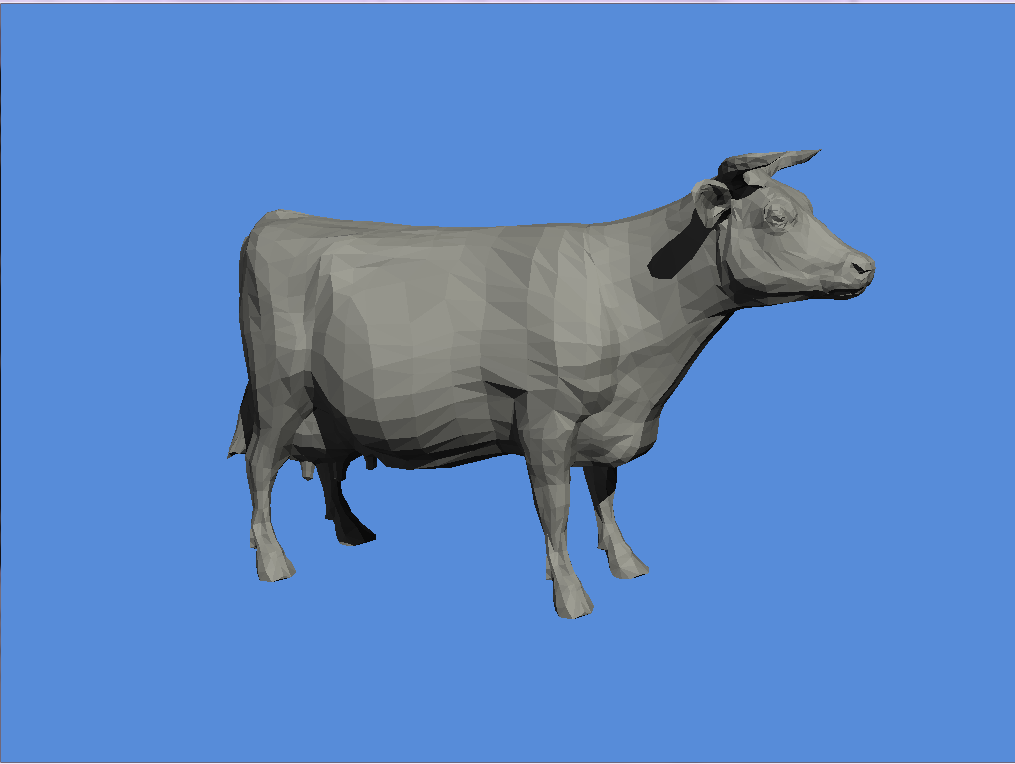
\includegraphics[width=0.5\linewidth]{my.png}}
\caption{Пример 2.}
\label{map}
\end{figure}